%----------------------------------------------------------------------------------------
%    PACKAGES AND THEMES
%----------------------------------------------------------------------------------------

\documentclass[aspectratio=169,12.5pt,xcolor=dvipsnames]{beamer}
\usetheme{SimpleDarkBlue}

\usepackage{hyperref}
\usepackage{graphicx} % Allows including images
\usepackage{booktabs} % Allows the use of \toprule, \midrule and \bottomrule in tables
\usepackage{caption}

%----------------------------------------------------------Alguns setups
%----------------------------------------------------------

%----------------------------------------------------------------------------------------
%    TITLE PAGE
%----------------------------------------------------------------------------------------

\title{Pré-relatório da segunda prática}
\subtitle{Constante de Planck}

\author{João Vítor Lima de Oliveira\\Guilherme Aranha}

\institute
{
    Instituto de Física de São Carlos
    \\
    Universidade de São Paulo % Your institution for the title page
}
\date{\today} % Date, can be changed to a custom date

%----------------------------------------------------------------------------------------
%    PRESENTATION SLIDES
%----------------------------------------------------------------------------------------

\begin{document}

\begin{frame}
    % Print the title page as the first slide
    \titlepage
\end{frame}

\begin{frame}{Sumário}
    % Throughout your presentation, if you choose to use \section{} and \subsection{} commands, these will automatically be printed on this slide as an overview of your presentation
    \tableofcontents
\end{frame}

%------------------------------------------------
\section{Motivação}
%------------------------------------------------

\begin{frame}{Motivação}
    \Huge{\centerline{\textbf{Motivação}}}
\end{frame}


\begin{frame}{Quantização da energia}

    \begin{columns}[c]
        \column{.45\textwidth}
        \begin{figure}
          \centering
          \caption{Max Planck}
          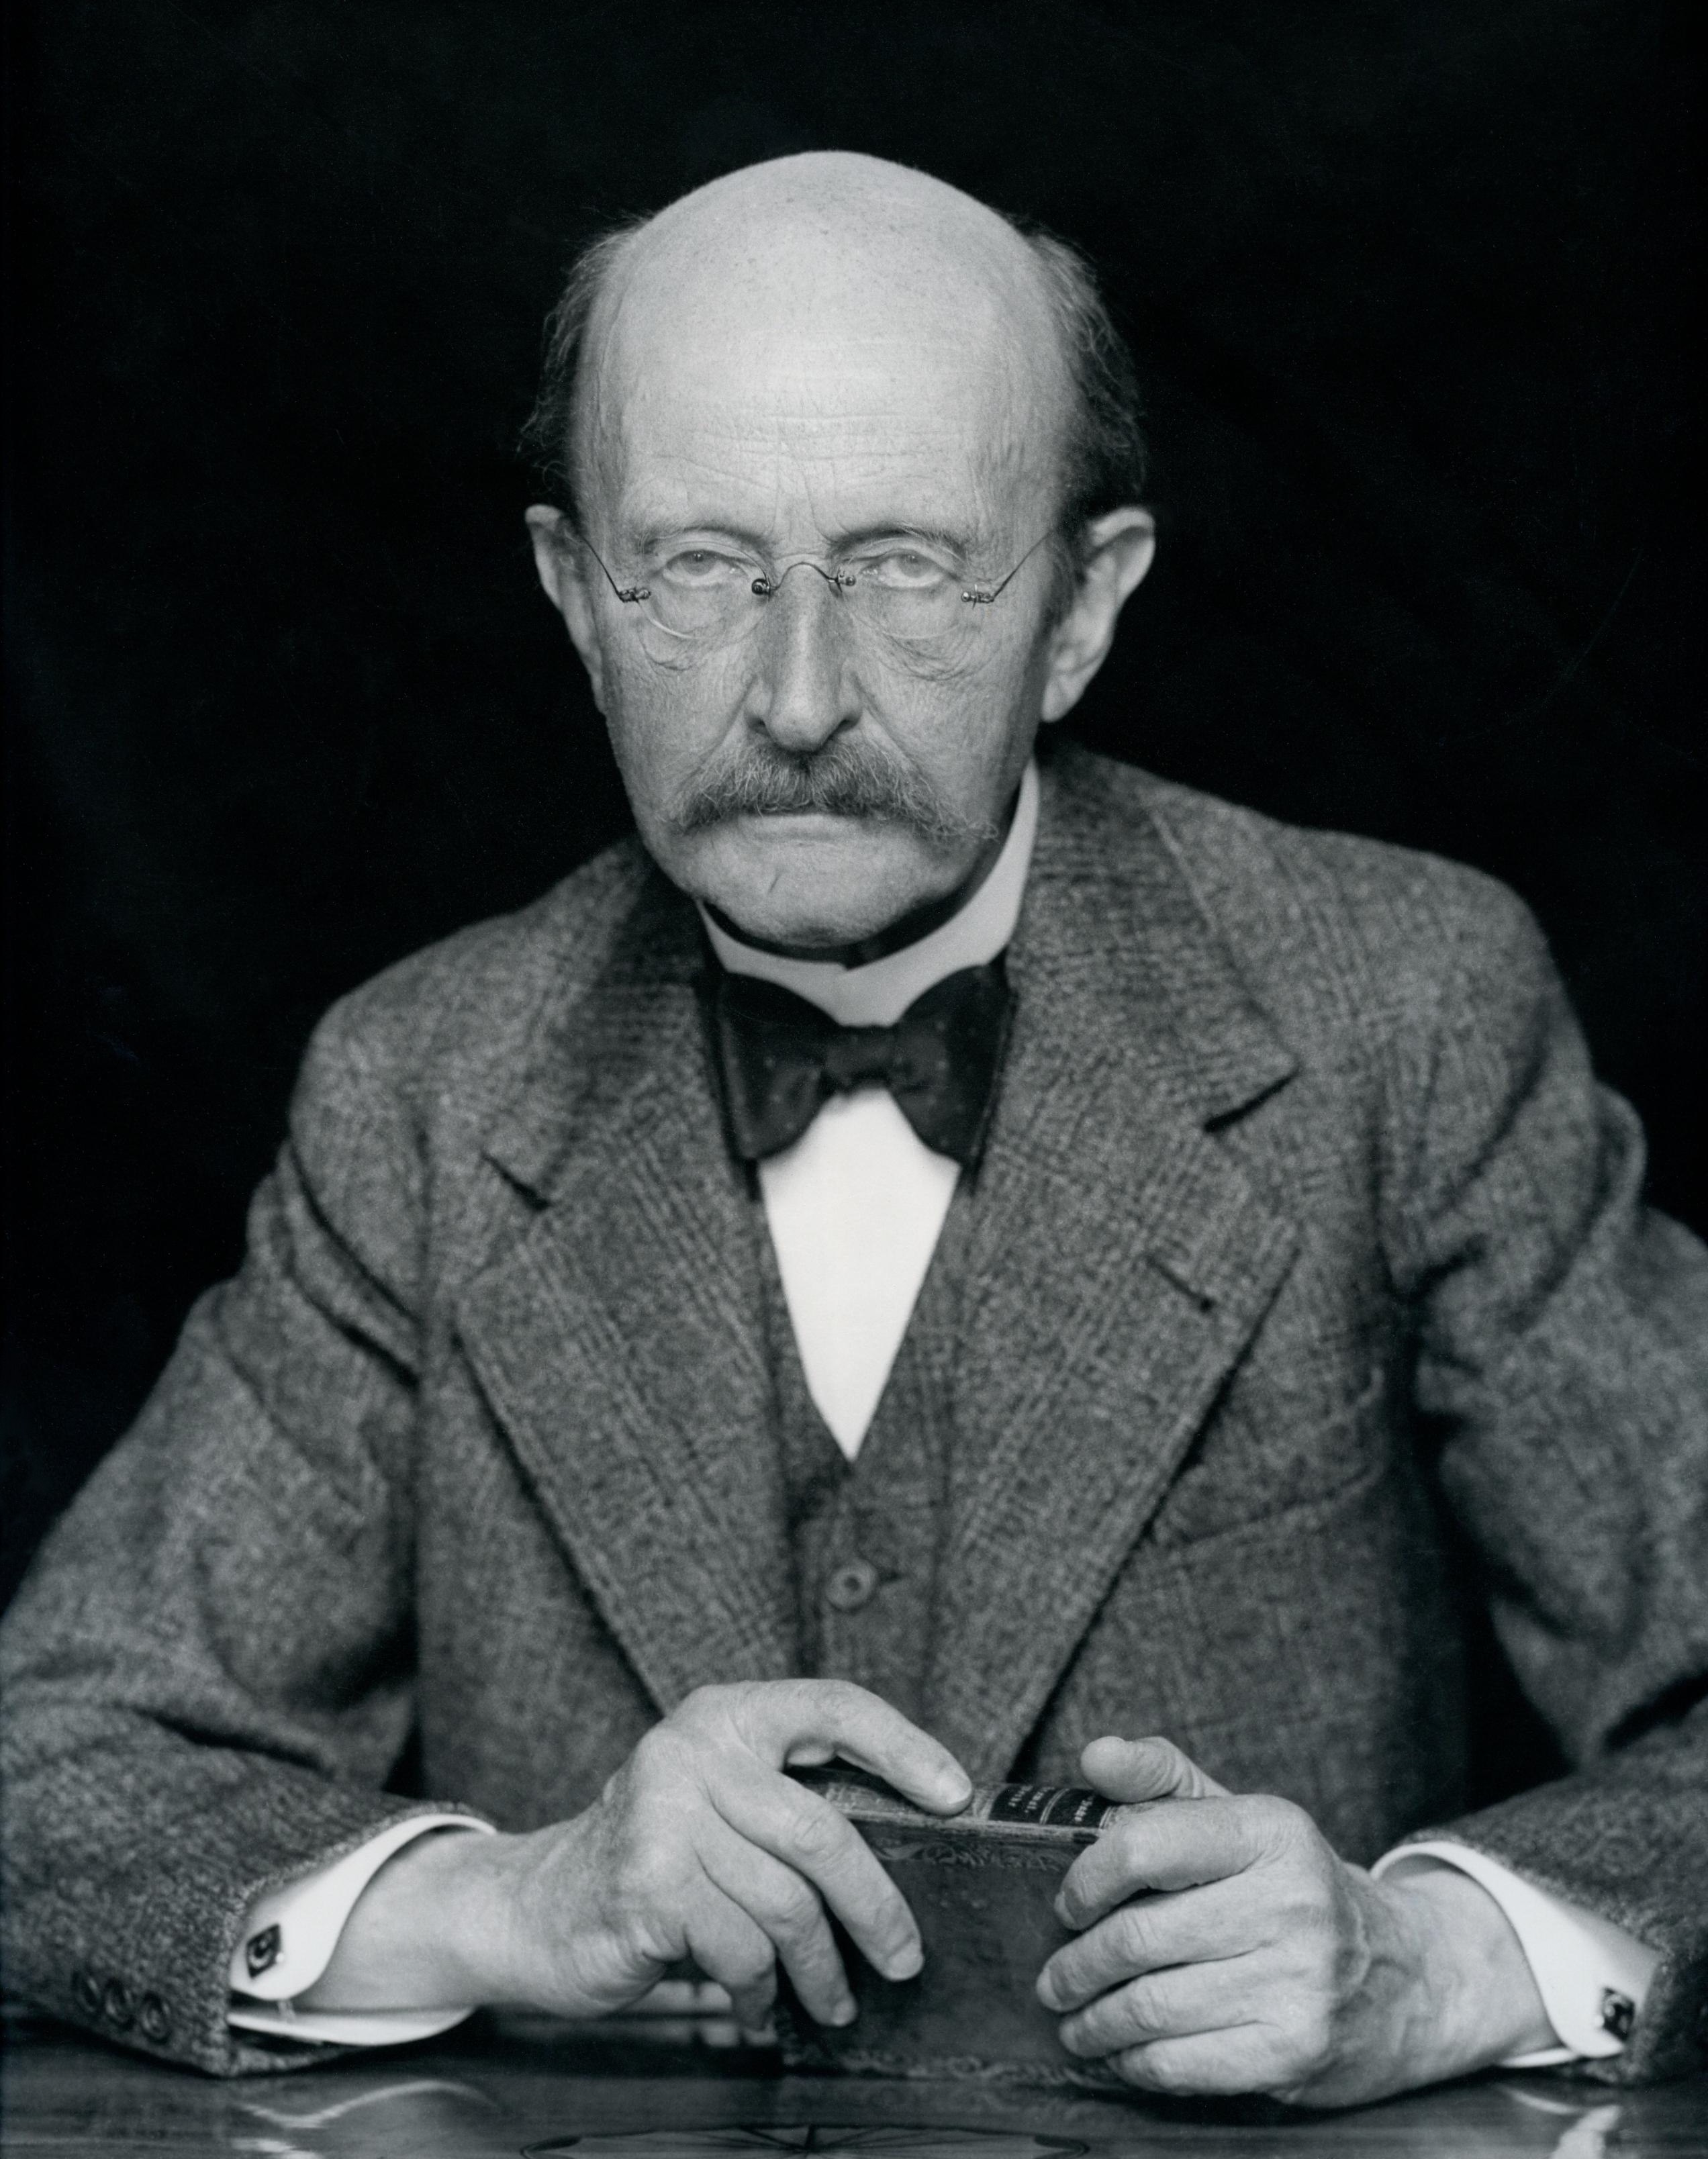
\includegraphics[width=4.25cm]{figuras/Planck.jpg}\par
          {\scriptsize Fonte: Retirado da internet.}
        \end{figure}

        \column{.45\textwidth}
        Em 1900, Max Planck utiliza a ideia de quantização da energia para resovler a Catástrofe Ultravioleta.
        \begin{equation}
            E = h\nu
        \end{equation}
    
    \end{columns}

    
\end{frame}

%------------------------------------------------

\begin{frame}{Catástrofe Ultravioleta}

        \begin{center}
        \begin{figure}
        \caption{Gráfico Iradiancia x Comprimento de Onda para um corpo negro.}
        \vspace*{-0.20cm}
        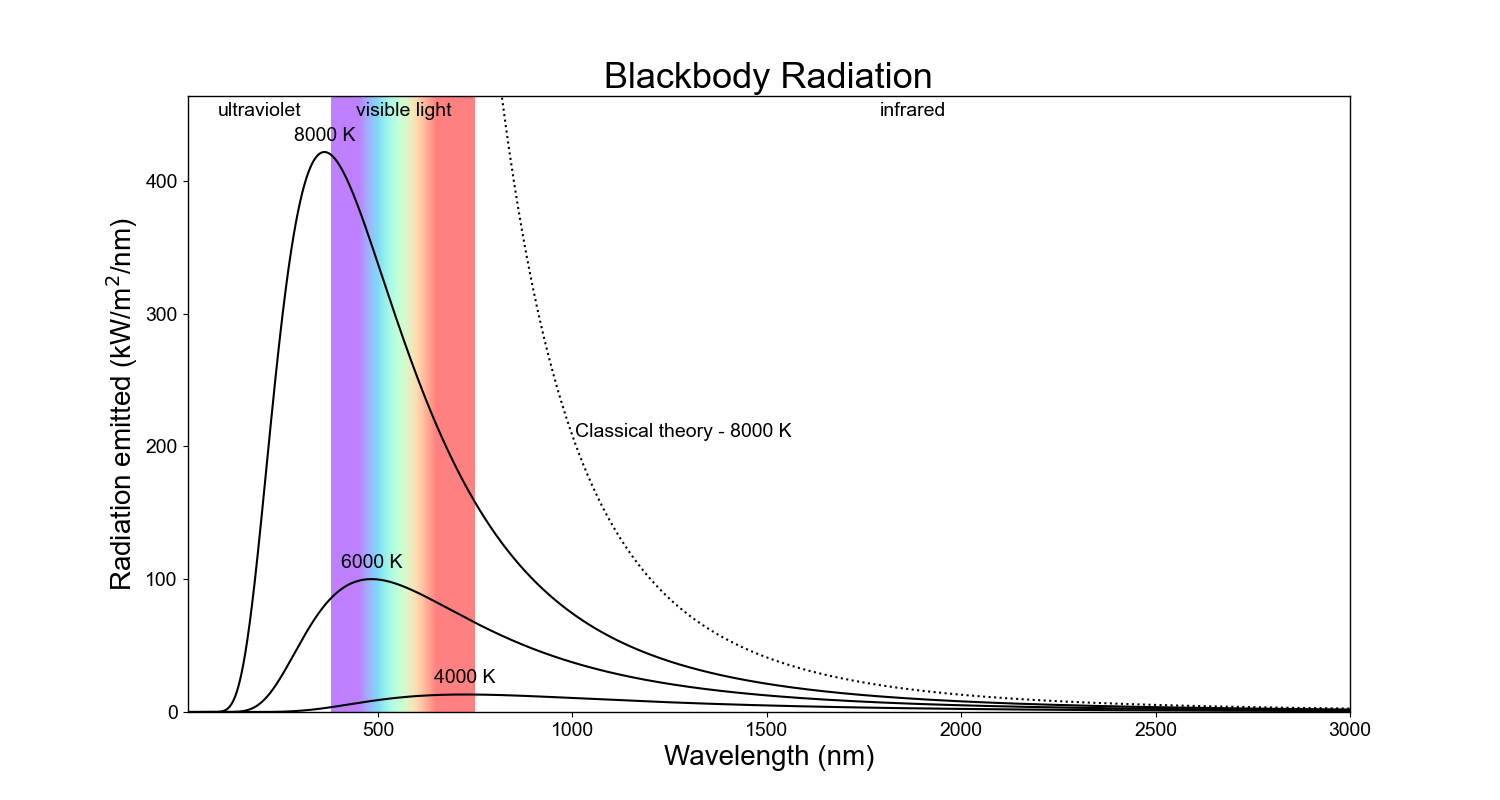
\includegraphics[width=0.75\textwidth,height=0.75\textheight,keepaspectratio]{figuras/Black_body.png}\par
        {\scriptsize Fonte: Retirado da internet.}
        \end{figure}
        \end{center}
    
\end{frame}


%------------------------------------------------
\section{Objetivos}
%------------------------------------------------
\begin{frame}{Objetivos}
    \Huge{\centerline{\textbf{Objetivos}}}
\end{frame}

\begin{frame}{Objetivos}

\vspace{1\baselineskip}

    \begin{itemize}
        \item Entender o princípio de funcionamento de um LED (light emitting diode).
        
        \item Estimar a constante de Planck $h$ a partir da tensão de limiar ($V_{min}$) para a qual um LED
passa a emitir luz.

        \item Comparar o valor de $h$ obtido com aquele estabelecido na literatura e discutir a respeito.
        
    \end{itemize}
\end{frame}
%------------------------------------------------
\section{Metodologia}
%------------------------------------------------
\begin{frame}{Metodologia}
    \Huge{\centerline{\textbf{Metodologia}}}
\end{frame}


\begin{frame}{Caracterização dos LED}

    \begin{columns}[c]
        \column{.60\textwidth}
        \begin{figure}
          \centering
          \caption{Curvas espectrais de um LED de estado sólido Azul e uma lampada incandescente.}
          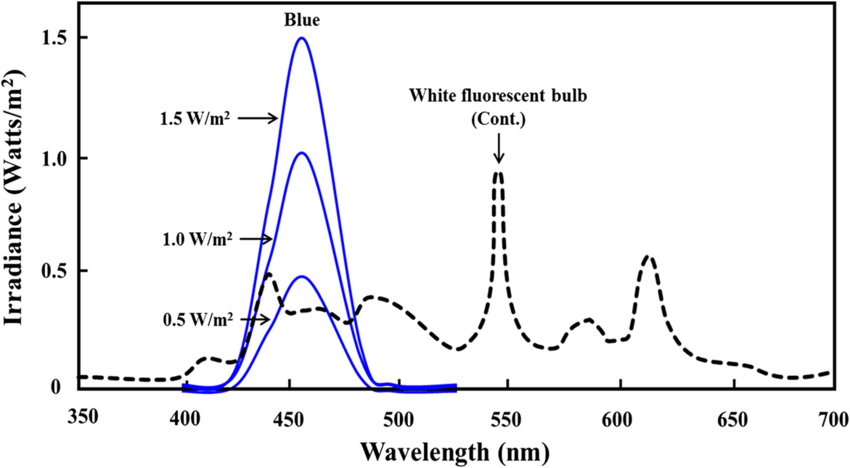
\includegraphics[width=0.85\textwidth,height=0.85\textheight,keepaspectratio]{figuras/led_blue.png}\par
          {\scriptsize Fonte: Retirado de \cite{Song2019}.}
        \end{figure}

        \column{.40\textwidth}

        Usaremos um espectrômetro para medir o comprimento de onda $\lambda$ emitido por cada LED.
    
    \end{columns}

    
\end{frame}

%------------------------------------------------

\begin{frame}{Caracterização dos LED}

    \begin{columns}[c]
        \column{.60\textwidth}
        \begin{figure}
          \centering
          \caption{Curvas $I\times V$ de LEDs de diferentes cores.}
          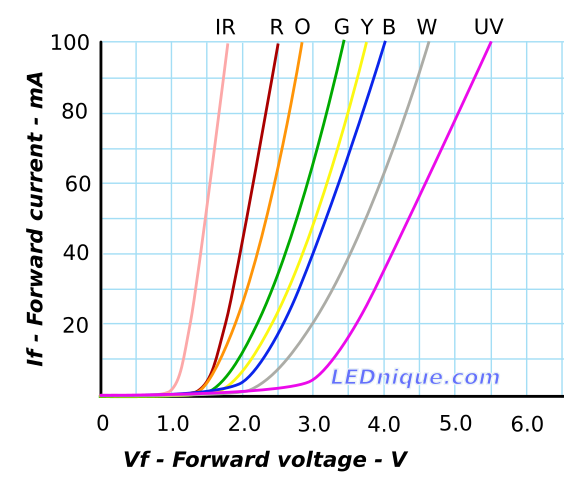
\includegraphics[width=0.75\textwidth,height=0.75\textheight,keepaspectratio]{figuras/IV-curves-all-colours.png}\par
          {\scriptsize Fonte: Retirado da internet.}
        \end{figure}

        \column{.40\textwidth}
        Aumentaremos a tensão em 0.10 V até encontrarmos a tensão, $V_{min}$ necessária para fazer o LED emitir Luz no visivel.
    
    \end{columns}


\end{frame}

%------------------------------------------------

\begin{frame}{}

Energia mínima para excítar elétrons da banda de Valência para a banda de condução $E_g$ está associado ao potencial aplicado pela equação.

\begin{equation}
    E_g = e V_{min} 
\end{equation}

então,

\begin{equation}
    V_{min} = \frac{E_g}{e} 
\end{equation}

usando a relação de Planck $E = h\nu$,

\begin{equation}
    h\nu = eV_{min} 
\end{equation}

\end{frame}

%------------------------------------------------

\begin{frame}{Método de ajuste Piecewise}

    \begin{columns}[c]
        \column{.60\textwidth}
        \begin{figure}
          \centering
          \caption{Exemplo do método Piecewise.}
          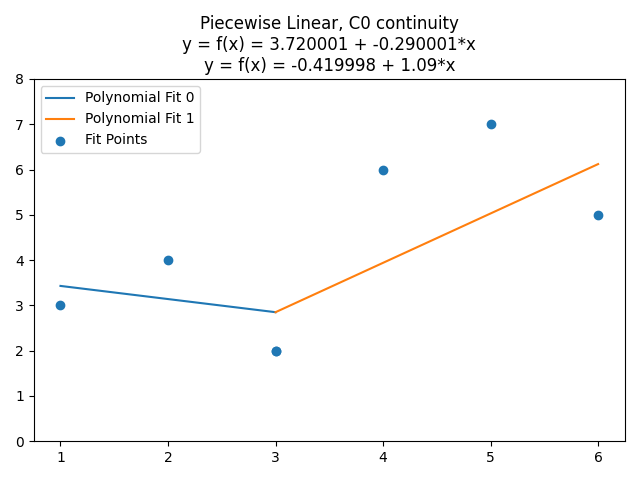
\includegraphics[width=0.85\textwidth,height=0.85\textheight,keepaspectratio]{figuras/picewise.png}\par
          {\scriptsize Fonte: Retirado da Internet.}
        \end{figure}

        \column{.40\textwidth}

        Usaremos o método de ajuste de curva Piecewise para encontrar o ponto onde $V_{min}$ na curva $I\times V$. O valor
estimatido de $V_{min}$ é dado pela intersecção das funções lineares.
    
    \end{columns}


\end{frame}


%------------------------------------------------
\section{Resultados esperados}
%------------------------------------------------

\begin{frame}{Resultados esperados}
    \Huge{\centerline{\textbf{Resultados esperados}}}
\end{frame}


\begin{frame}{Resultados}

Esperamos conseguir um valor para a constante de Planck que esteja na mesma ordem de grandeza $10^{-34}$ ou perto do valor estabelecido de $6.62607015 \times 10^{-34} $[J$\cdot$s]. Faremos a analise do nossos resultados utilizando a equação,


\begin{equation}
    h = \frac{eV_{min}}{\nu} 
\end{equation}

já que sabemos a frequência $\nu$ e a tensão mínima, $V_{min}$ para diferentes LEDs. Com várias amostragens, seremos capazes de encontrar um valor aproximado de $h$.
\end{frame}

%------------------------------------------------

\begin{frame}{References}
    \footnotesize
    \bibliography{reference.bib}
    \bibliographystyle{apalike}
\end{frame}

%------------------------------------------------

\begin{frame}
    \Huge{\centerline{\textbf{Obrigado!}}}
\end{frame}

%----------------------------------------------------------------------------------------

\end{document}